\setcounter{page}{1}
\section*{Introduction}
Due to their small dimensions, high efficiency, tunability and compatibility 
with electronic components, diode lasers are of great economical and scientifical interest . This experiment (\emph{V60 Diode Laser Physics}) aims to get familiar
with the calibration and frequency modulation of a diode laser. After a preparation the given setup enables us to measure
the absorption spectrum of gaseous Rubidium.

\section{Theory}
In the following we will present the theoretical background to understand how the experiment works. 
For this we follow the manual~\cite{anleitung60} and source~\cite{eichler}.

\subsection{Functionality of lasers}
Lasers are sources of monochromatic, intensive and especially \textbf{coherent} light.
To understand how a laser works it is firstly necessary to discuss the most fundamental interactions between light and
a quantum mechanical system like an atom. Figure~\ref{fig: two_level} shows a two level energy scheme. An electron in the
lowest state can be stimulated into the highest state by absorbing an incoming photon (Figure~\ref{fig: two_level} a). The relaxtion back into the
ground state can be radiative or nonradiative. 
The emission of a photon can be \textbf{spontaneous} (Figure~\ref{fig: two_level} b)
or \textbf{induced} by an incoming photon (Figure~\ref{fig: two_level} c). 
After that the two photons have the same direction, energy and phase.
That is why the so called \textbf{induced emission} is the crucial process for lasers. To increase the propability of the induced emission in
comparison to the absorption, the population of the second state has to be higher than the ground state. This is called
\textbf{inversion of population}.

\begin{figure}
  \centering
  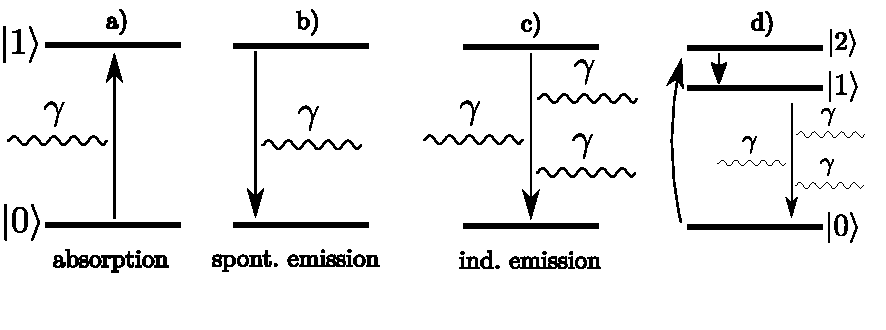
\includegraphics[scale = 0.9]{pics/energyscheme.pdf}
  \caption{Energy schemes to introduce the most fundamental interactions of light with a quantum mechanical system. Figures a) - c) show
  a two level system with the three processes absorption, spontaneous emission and induced emission. d) illustrates the easiest possible lasing
  system with three energy levels.}
  \label{fig: two_level}
\end{figure}

It is worth mentioning that the two level model is not a possible lasing system because an inversion of population
can not be achieved. That can for example be understood
regarding the population propability $p_2$ of the state $|2\rangle$
\begin{equation}
  p_2 = \frac{e^{-\frac{E_2}{k_B T}}}{ e^{-\frac{E_1}{k_B T}} + e^{-\frac{E_2}{k_B T}} } =
  \frac{1}{ e^{-\frac{E_1 - E_2}{k_B T}} + 1}
    \quad \underset{T \rightarrow \infty}{\longrightarrow}\quad  \frac{1}{2},
\end{equation}
with the temperature $T$ and the Boltzmann constant $k_B$. We see that one can achieve at most an equal population. The easiest
realistic system is a three level energy scheme (Figure~\ref{fig: two_level} d). Here it is important that the lifetime of the highest state $\tau_2$ is much shorter
than the lifetime $\tau_1$ of the first excited level ($\tau_2 \ll \tau_1$). By exciting electrons from the ground state into the highest
state an inversion of population between the first state and the ground state can be realised.

In general lasers consist of a laser medium, a optical cavity and a pump source (see figure~\ref{fig: principle_laser}).
The laser medium could be a gas (prominent example is a mixture of helium and neon) with electronic states like discussed above. The pump source
creates an inversion of population in the medium. The cavity consists of two mirrors that make the light pass several times through the medium, before
it leaves the system. For that, one of the mirrors has to be partial transparent (reflectivity slightly under \SI{100}{\percent}). In the
cavity only discrete \textbf{longitudinal modes}, which are given by the length of the cavity $L$ are allowed (analogous 
to the wavelength of standing waves of a rope that is fixed on both sides). In terms of wavelength these are
given by
\begin{equation}
  \lambda_m = \frac{2 L n}{m}
  \label{eq: standing_waves}
\end{equation}
where $c$ is the vacuum speed of light and $n$ the refractive index of the medium. Equation~\eqref{eq: standing_waves} shows that a manipulation of the
cavity length allows to select different laser wavelengths. The wavelength distribution defined by the optical transitions in the medium 
are typically much broader than the distance $\Delta \lambda$ between to longitudinal modes. 

\begin{figure}
  \centering
  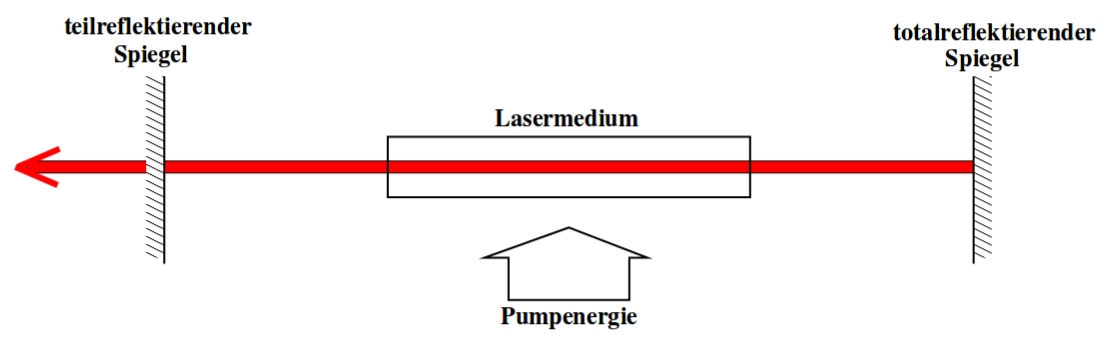
\includegraphics[width = 0.7\textwidth]{pics/prinzip_laser.png}
  \caption{Principle of a laser consisting of a medium, a pump source and a cavity. The cavity is here realised by two mirrors.
  Picture from \cite{anleitung61}, text translated.}
  \label{fig: principle_laser}
\end{figure}

\subsection{Functionality of diode lasers}
We now explain how the general concepts of a laser are realised in a diode laser. Here a semiconductor serves as the medium and a current as the pump source.
Often there are two cavities: the \textbf{internal cavity} is given by the reflecting interfaces of the medium, an \textbf{external cavity} consist of
a semiconductor interface at one side and a grating at the other. These three parts of the laser will be discussed more closely in the following.

In general a semiconductor is a solid with a finite bandgap $E_g$ between valence and conduction band. A hetero structure of \ce{AlGaAs} ($p$-doped),
\ce{GaAs} ($n$-doped)
and \ce{AlGaAs} ($p$-doped) leads to a band scheme like shown in figure~\ref{fig: bandstructure}. 
\begin{figure}
  \centering
  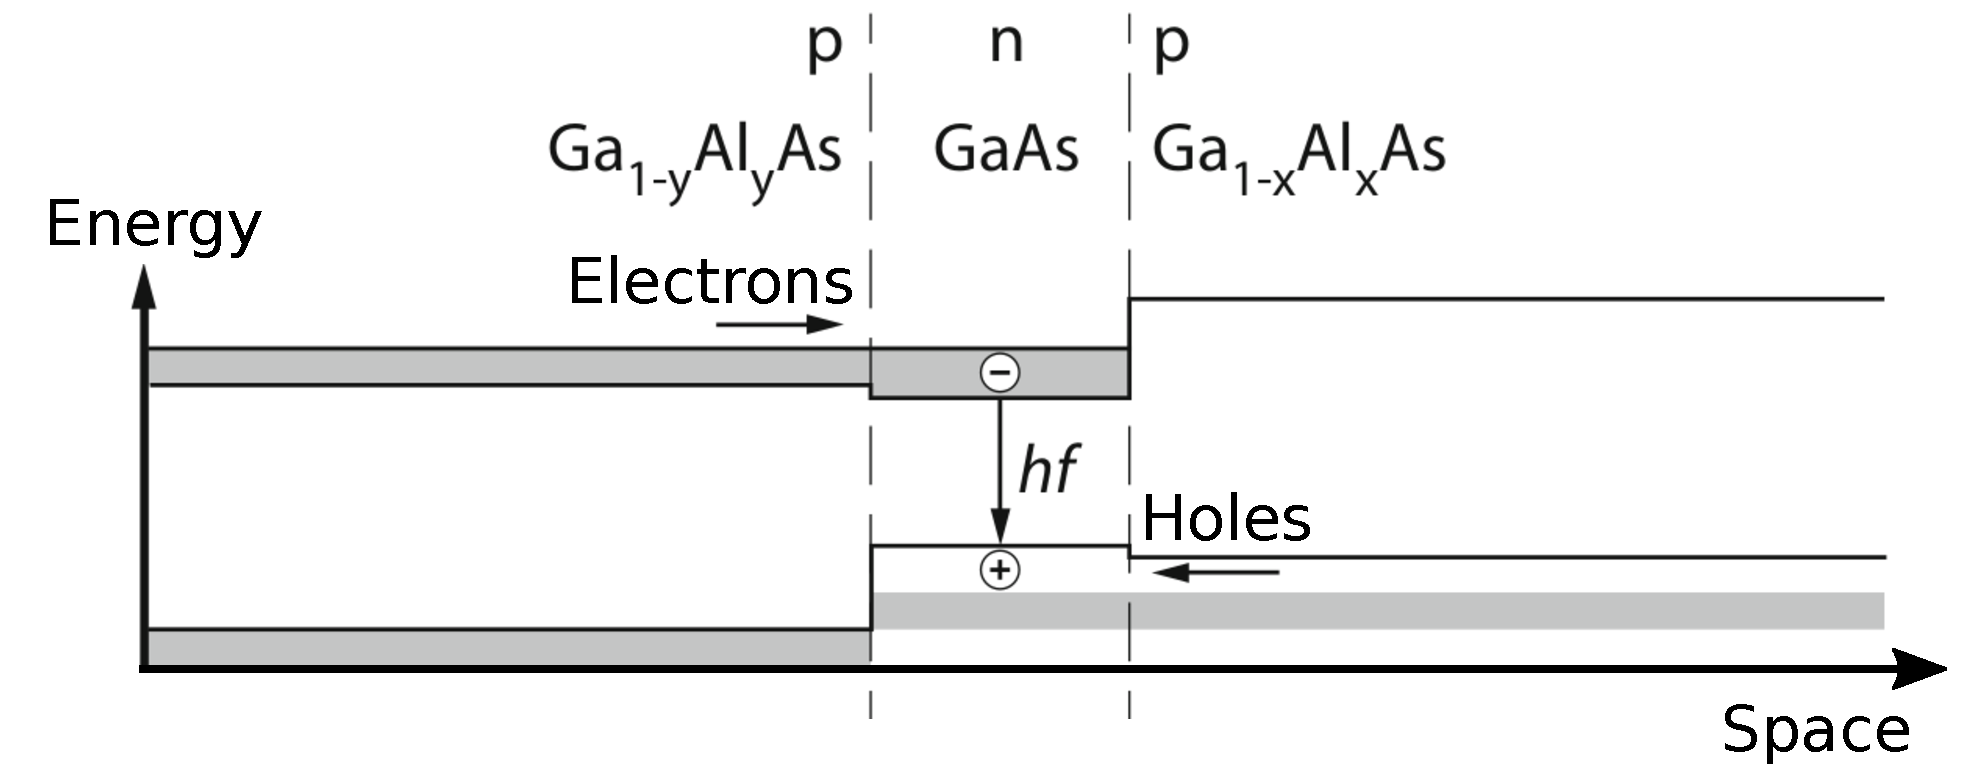
\includegraphics[width = 0.7\textwidth]{pics/hetero_structure.pdf}
  \caption{Energy scheme of an \ce{AlGaAs}-\ce{GaAs} hetero structure. Picture from \cite{eichler}, text edited.}
  \label{fig: bandstructure}
\end{figure}
The electrons and holes see a potential well
in the \ce{GaAs} layer, which is the active zone of the laser. The current induced by an applied voltage increases the number of electrons
and holes in the conduction and valence band respectively. Due to the fact, that \ce{GaAs} is a direct semiconductor, electrons and holes can
recombine efficiently by emmiting a photon with energy $E_g$ ($E_g = hf$ in figure~\ref{fig: bandstructure}). A typical plot of laser intensity versus current is shown in figure~\ref{fig: threshold}. For low
currents the laser acts similar to a light emmiting diode (LED) and the intensity is small. Above a threshold $I_{th}$ the intensity rises rapidly.
From this point losses inside the cavity are compensated and induced emission begins. Nevertheless, the intensity is limited by joule heating
of the diode (see figure~\ref{fig: threshold}). Since the bandgap $E_g = E_g(T)$ decreases with temperature, varying the current affects
the wavelength of the laser because of heating as well.



\begin{figure}
  \centering
  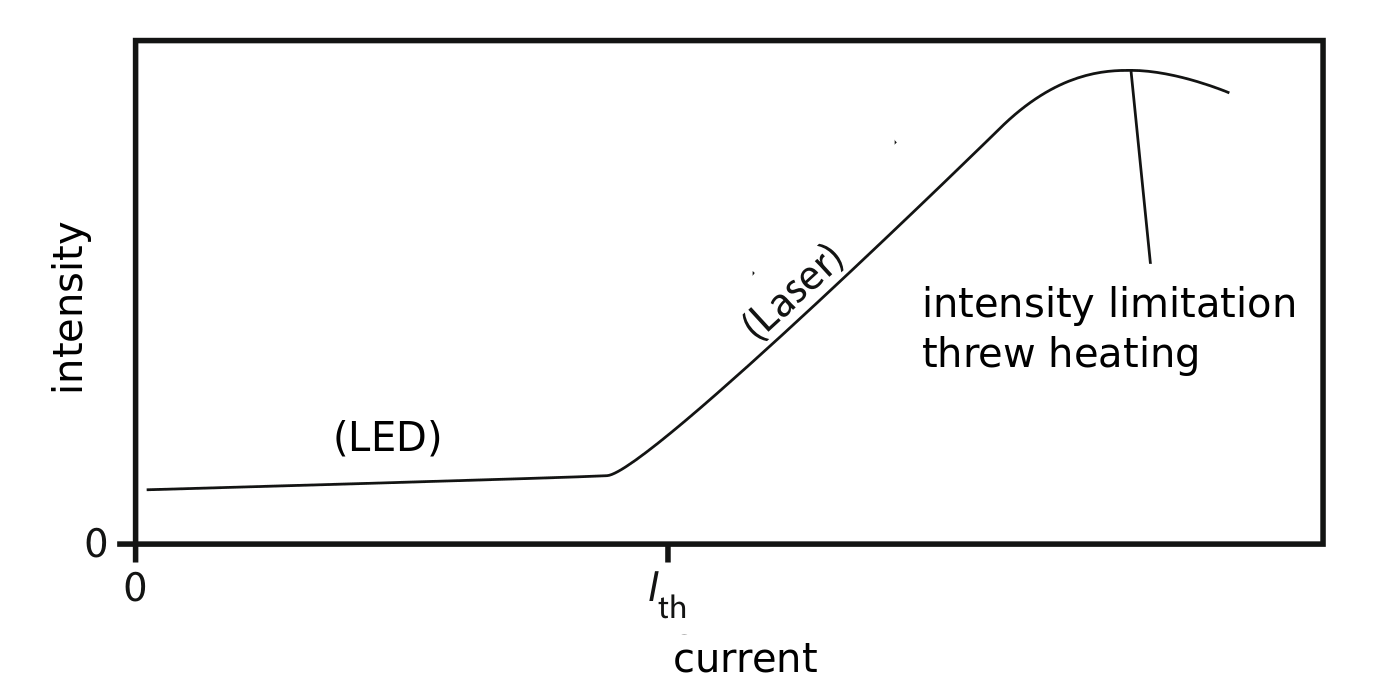
\includegraphics[width = 0.7\textwidth]{pics/threshold.png}
  \caption{Typical realtion between laser current and output intensity of a diode laser. From a threshold current 
  $I_{th}$ the system begins to lase. Picture from \cite{eichler}, text edited.}
  \label{fig: threshold}
\end{figure}

The photons pass the active zone several times because of the cavities and induce further emissions. A typical alignment is displayed in figure~\ref{fig: cavity}.
A collimating lens behind the medium is necessary because the light from the thin active zone is strongly diverging (most 
fundamental reason for that is Heisenbergs uncertainty principle).
Like mentioned before the external cavity has an optical grating on one side. The grating is set so that the first diffrection maximum is send back into the
diode. Because of the dispersive effect of the grating, the wavelength can be selected by rotating the grating around an axis perpenducular
to the image surface. Regarding equation~\eqref{eq: standing_waves} the longitudanal modes of the external cavity are much
more closely to each other than the ones of the internal cavity ($\Delta \lambda \sim 1 / L$).
To modulate the laser frequency either the length of the extrenal cavity or the current can be varied.
Changing only the external cavity length or the angle of the grating can lead to \textbf{mode hops}, when the overall gain becomes higher
in a diffrent internal mode. By a simultaneous variation of the laser current and the external cavity length mode hops can be avoided.

\begin{figure}
  \centering
  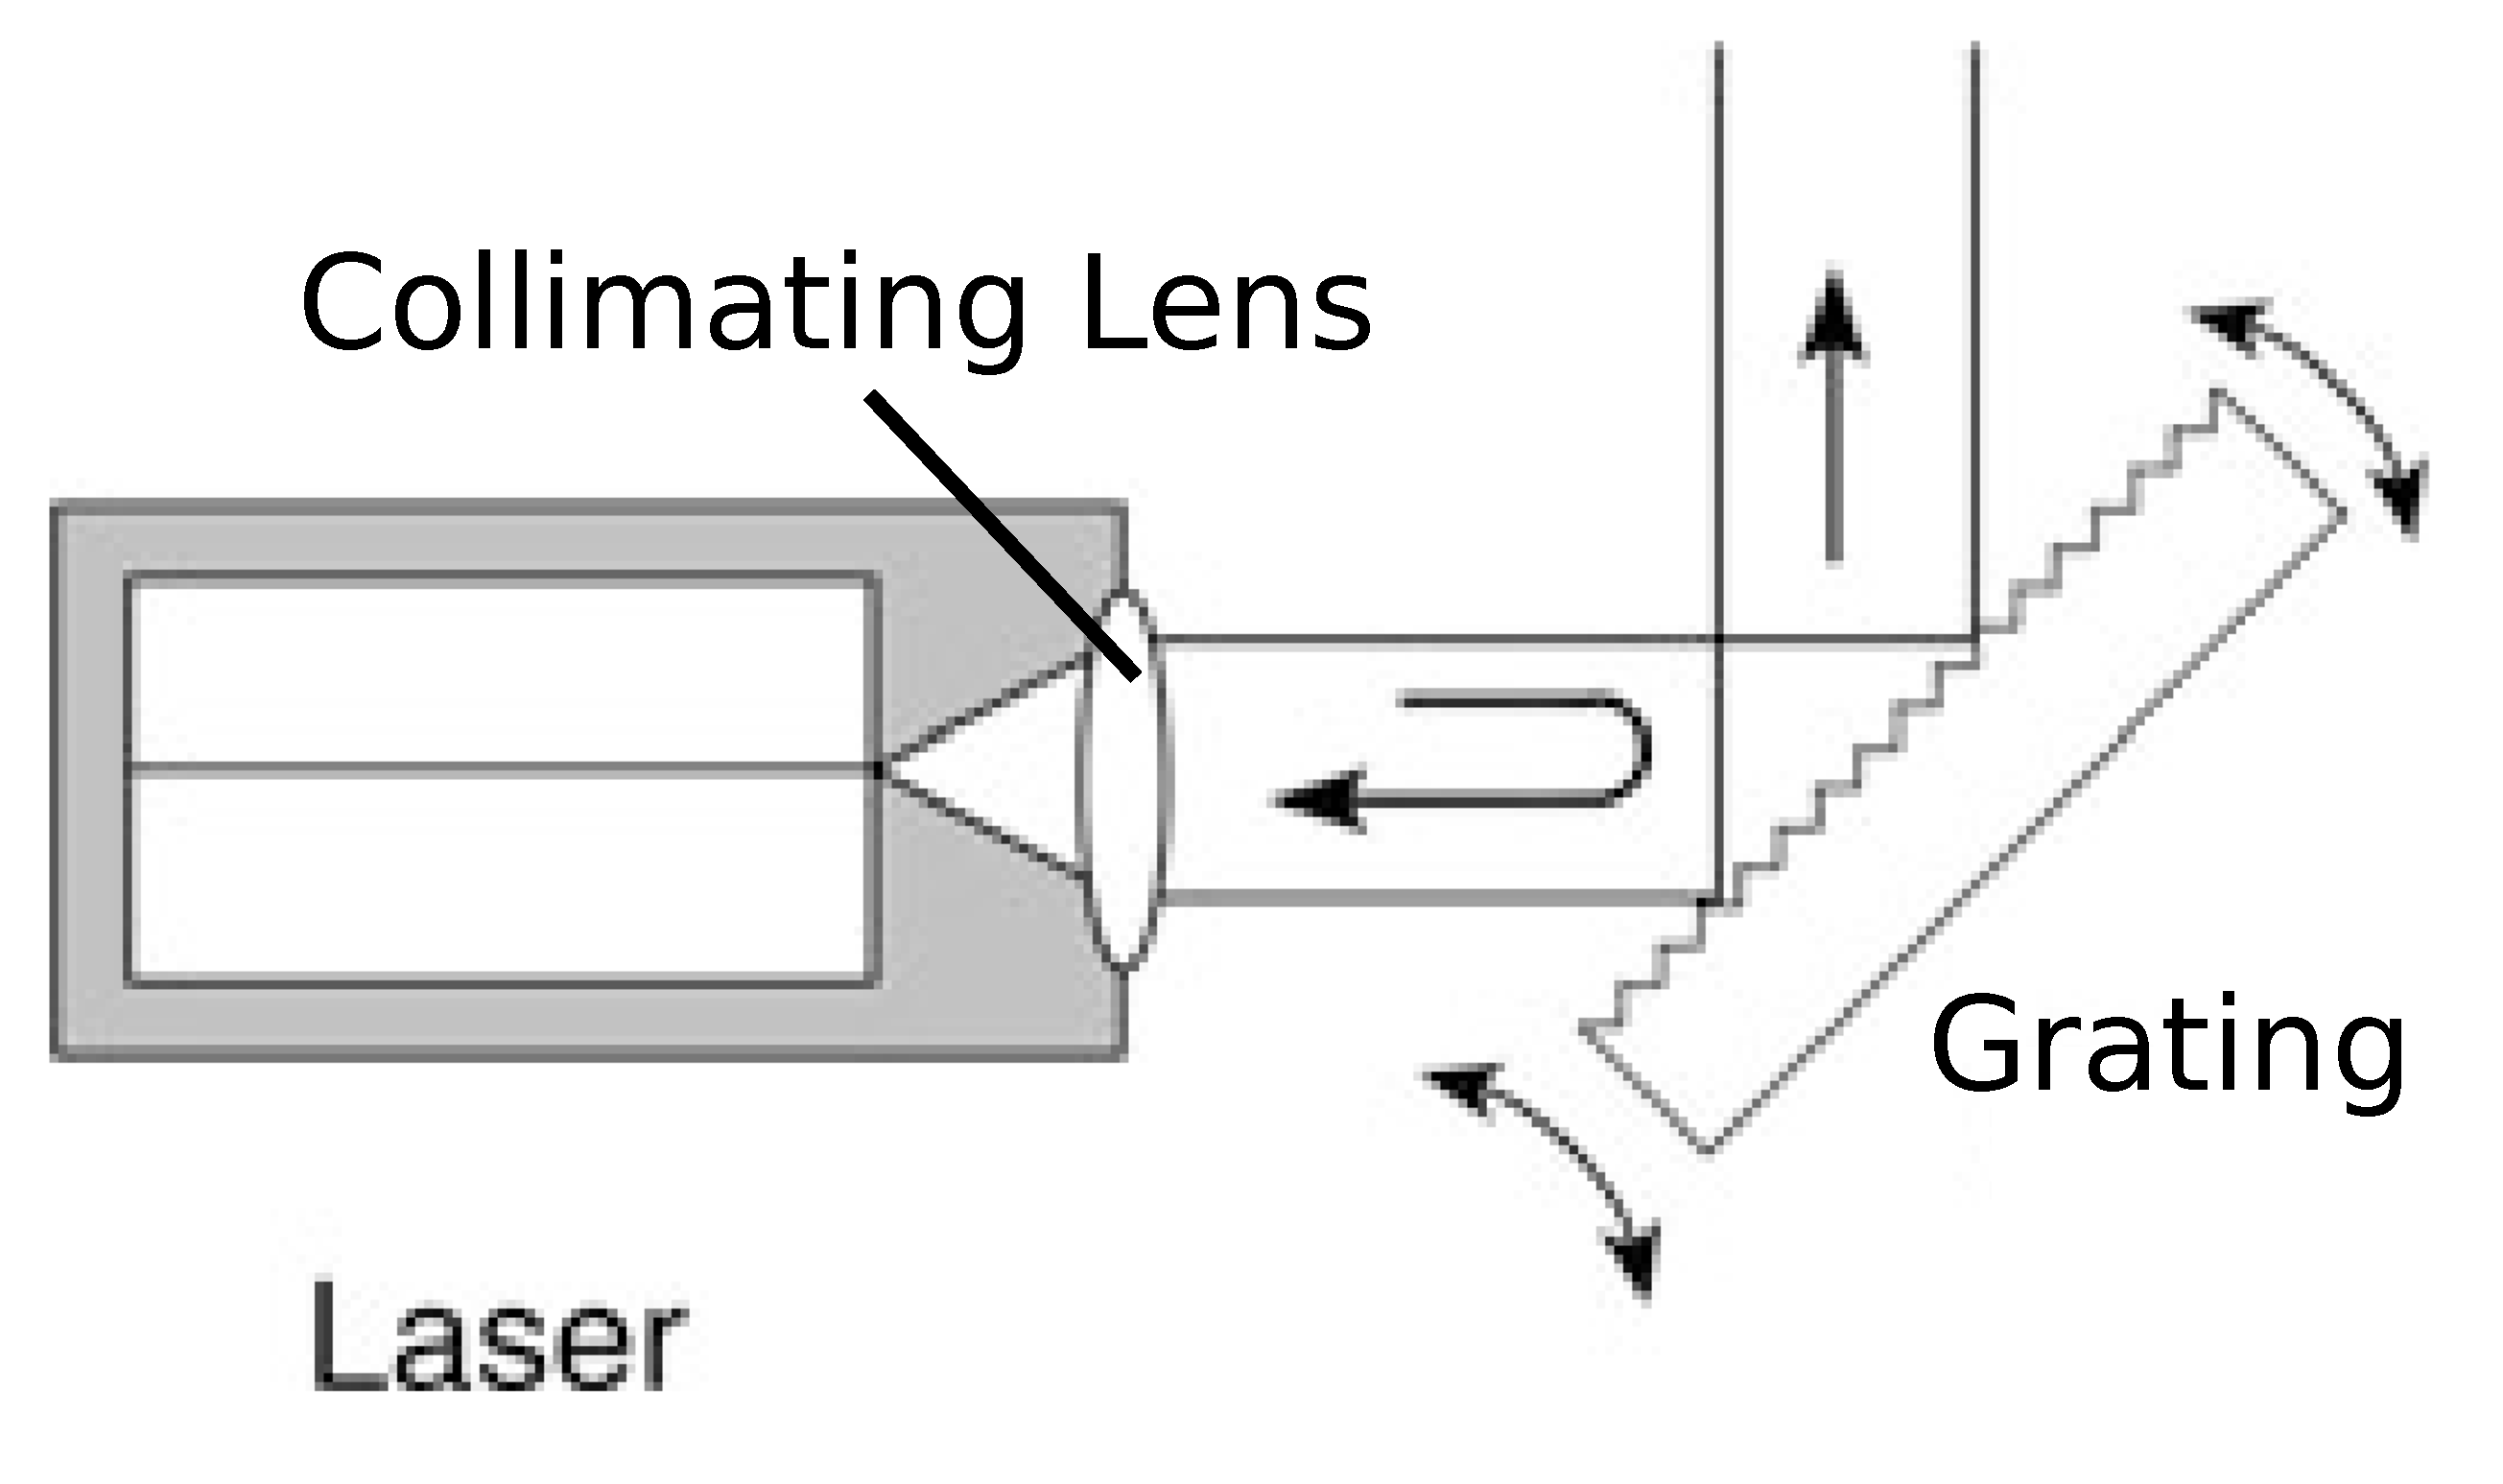
\includegraphics[width = 0.5\textwidth]{pics/cavity.pdf}
  \caption{Typical alignment of diode laser including a external cavity. 
  Picture from \cite{eichler}, text edited.}
  \label{fig: cavity}
\end{figure}
